\chapter{Pointers}
\myindex{\CLanguageElements!\Pointers}
\label{label_pointers}

Pointers are often used to return values from functions (recall \scanf case~(\myref{label_scanf})).

For example, when a function needs to return two values.

\section{Global variables example}

\lstinputlisting{patterns/061_pointers/global.c}

This compiles to:

\lstinputlisting[caption=\Optimizing MSVC 2010 (/Ob0)]{patterns/061_pointers/global.asm}

\myindex{\olly}
\clearpage
Let's see this in \olly:

\begin{figure}[H]
\centering
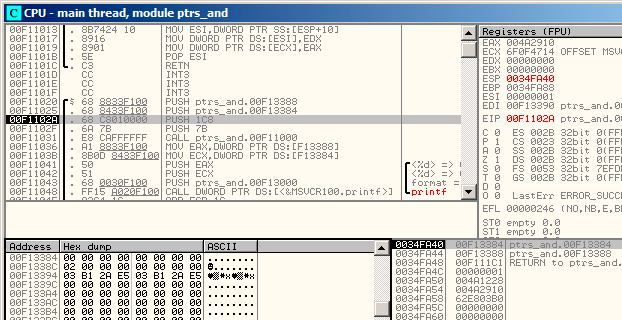
\includegraphics[scale=\FigScale]{patterns/061_pointers/olly_global1.png}
\caption{\olly: 
global variables addresses are passed to \ttfone}
\label{fig:pointers_olly_global_1}
\end{figure}

First, global variables' addresses are passed to \ttfone.
We can click \q{Follow in dump} 
on the stack element, and we can see the place in the data segment allocated 
for the two variables.

\clearpage
These variables are zeroed, because non-initialized data (from \ac{BSS}) is cleared before
the execution begins: [\CNineNineStd 6.7.8p10].

They reside in the data segment, we can verify this by pressing Alt-M and reviewing the memory map:

\begin{figure}[H]
\centering
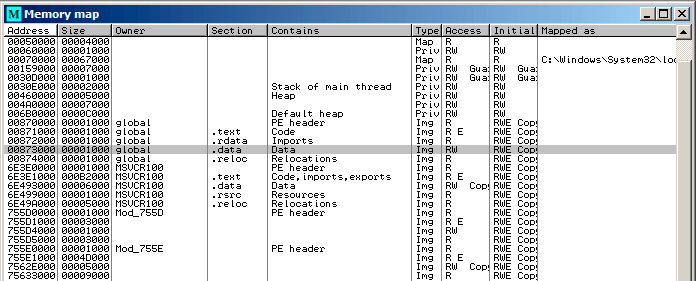
\includegraphics[scale=\FigScale]{patterns/061_pointers/olly_global5.png}
\caption{\olly: memory map}
\label{fig:pointers_olly_global_5}
\end{figure}

\clearpage
Let's trace (F7) to the start of \ttfone: 

\begin{figure}[H]
\centering
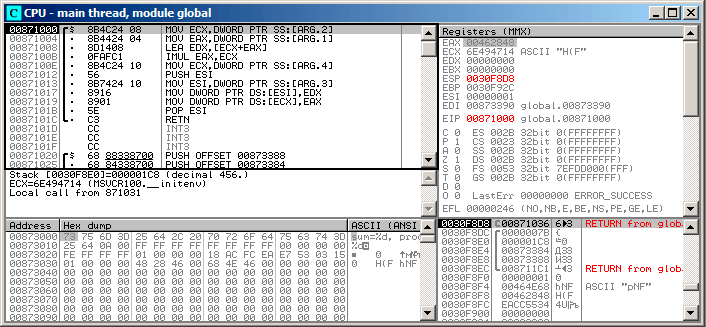
\includegraphics[scale=\FigScale]{patterns/061_pointers/olly_global2.png}
\caption{\olly: \ttfone starts}
\label{fig:pointers_olly_global_2}
\end{figure}

Two values are visible in the stack 456 (\TT{0x1C8}) and
123 (\TT{0x7B}), and also the addresses of the two global variables.

\clearpage
Let's trace until the end of \ttfone.
In the left bottom window we see how the results of the calculation appear in the global variables: 

\begin{figure}[H]
\centering
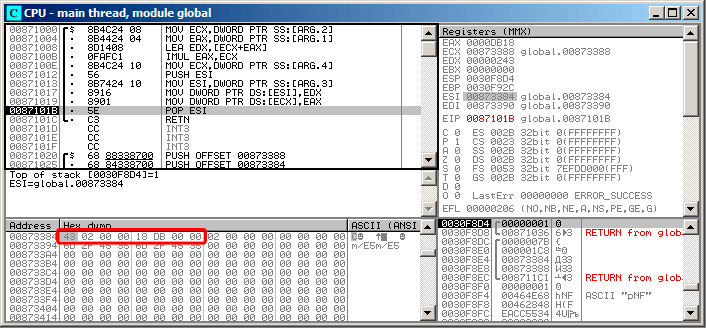
\includegraphics[scale=\FigScale]{patterns/061_pointers/olly_global3.png}
\caption{\olly: \ttfone execution completed}
\label{fig:pointers_olly_global_3}
\end{figure}

\clearpage

Now the global variables' values are loaded into registers ready for passing to \printf (via the stack):

\begin{figure}[H]
\centering
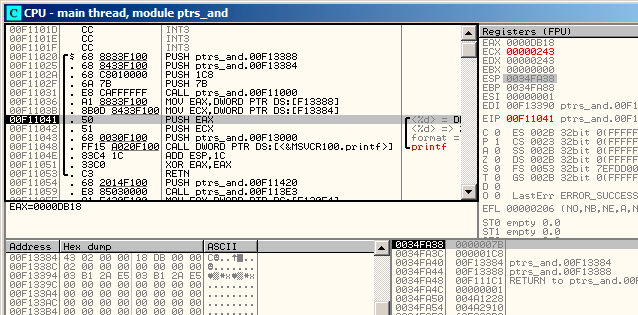
\includegraphics[scale=\FigScale]{patterns/061_pointers/olly_global4.png}
\caption{\olly: 
global variables' addresses are passed into \printf}
\label{fig:pointers_olly_global_4}
\end{figure}

\section{Local variables example}

Let's rework our example slightly:

\lstinputlisting[caption=now the \TT{sum} and \TT{product} variables are local]{patterns/061_pointers/local_EN.c}

\ttfone code will not change.
Only the code of \main will do:

\lstinputlisting[caption=\Optimizing MSVC 2010 (/Ob0)]{patterns/061_pointers/local.asm}

\newcommand{\PtrsAddresses}{\TT{0x2EF854} \AndENRU \TT{0x2EF858}\xspace}

\clearpage
Let's look again with \olly.
The addresses of the local variables in the stack are \PtrsAddresses.
We see how these are pushed into the stack: 

\begin{figure}[H]
\centering
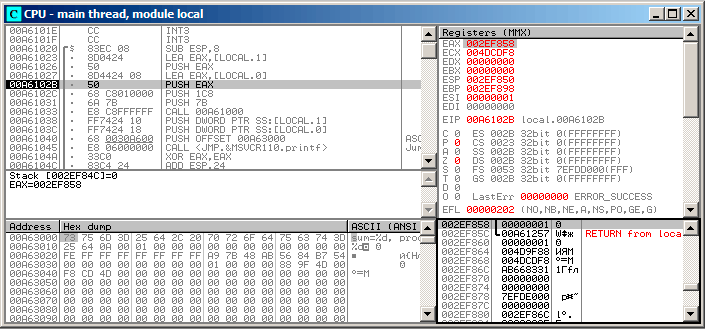
\includegraphics[scale=\FigScale]{patterns/061_pointers/olly_stk1.png}
\caption{\olly: local variables' addresses are
pushed into the stack}
\label{fig:pointers_olly_stk_1}
\end{figure}

\clearpage
\ttfone starts.
So far there is only random garbage in the stack at \PtrsAddresses :

\begin{figure}[H]
\centering
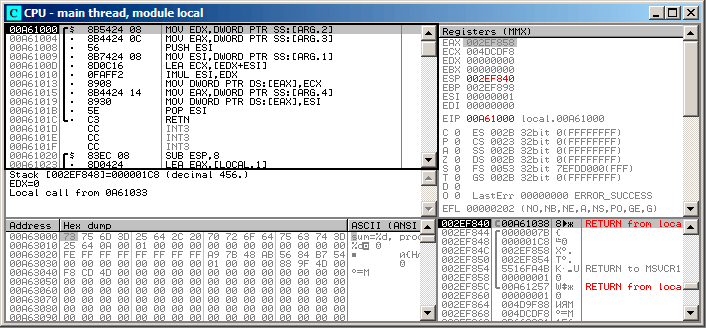
\includegraphics[scale=\FigScale]{patterns/061_pointers/olly_stk2.png}
\caption{\olly: \ttfone starting}
\label{fig:pointers_olly_stk_2}
\end{figure}

\clearpage
\ttfone completes:

\begin{figure}[H]
\centering
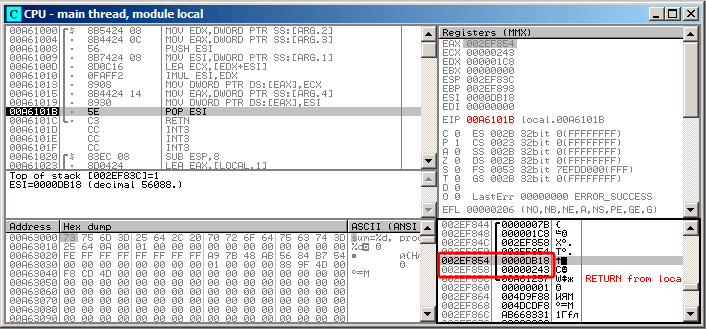
\includegraphics[scale=\FigScale]{patterns/061_pointers/olly_stk3.png}
\caption{\olly: \ttfone completes execution}
\label{fig:pointers_olly_stk_3}
\end{figure}

We now find \TT{0xDB18} and \TT{0x243} at addresses \PtrsAddresses.
These values are the \ttfone results.

\section{\Conclusion{}}
 
\ttfone could return pointers to any place in memory, located anywhere.

This is in essence the usefulness of the pointers.

By the way, \Cpp \IT{references} work exactly the
same way. Read more about them: (\myref{cpp_references}).
